\chapter{Novo modelo Denavit-Hartenberg}

\label{apendice-dh}

Seguindo a convenção adotada para o trabalho, o primeiro sistema de coordenadas a ser posicionado 
deve ser o da junta 1. 
Através da figura \ref{fig:a1} nota-se que os eixos das juntas 1 e 2 não se interceptam, portanto a 
origem deve ser posicionada no ponto de intersecção entre a perpendicular comum aos eixos das juntas 1 e 2,
e o eixo da junta 1, equivalente ao quadrado verde na figura.
O eixo $\hat{Z}_1$ foi posicionado na direção do eixo da junta $1$, com sentido para fora do plano da imagem,
e o eixo $\hat{X}_1$ na direção da perpendicular comum, com sentido do eixo da junta 1 para o eixo da junta 2.
Na figura a distância mostrada faz referência ao parâmetro $a_1$.

\begin{figure}[ht]
    \caption{Distância entre os eixos das juntas 1 e 2.}    
    \begin{centering}

        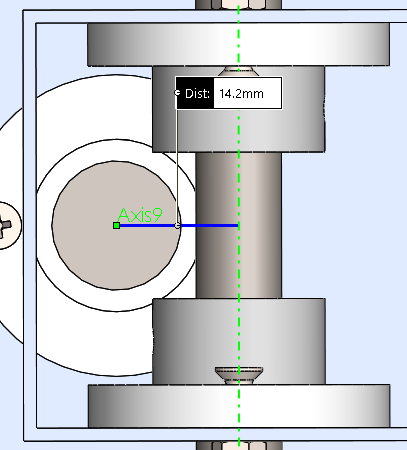
\includegraphics[width=0.5\columnwidth]{adendo/images/a1.png}
    
    \par\end{centering}

    \label{fig:a1}
\end{figure}

Seguindo os passos de 2 a 5 descritos na seção \ref{sec:fundamentos-dh} foram definidos também os sistemas
de coordenadas das juntas de 2 a 5, resultando nos parâmetros $a_2$, $a_3$ e $a_4$. Os valores para estes
termos podem ser vistos nas figuras de \ref{fig:a2} a \ref{fig:a4}. 
Vale a pena notar que para a junta 5, os eixos $\hat{Z}_5$ e $\hat{Z}_6$ se interceptam, como pode ser
visto na figura \ref{fig:d6}, portanto o eixo $\hat{X}_5$ foi definido na direção da reta normal ao plano 
formado por esses dois eixos $\hat{Z}$.  

\begin{figure}[ht]
    \caption{Distância entre os eixos das juntas 2 e 3.}    
    \begin{centering}

        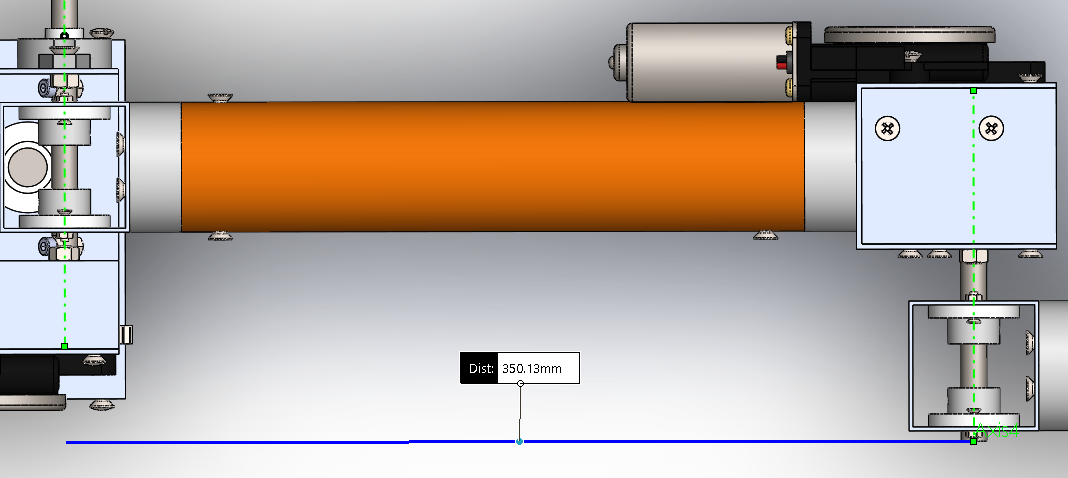
\includegraphics[width=0.9\columnwidth]{adendo/images/a2.png}
    
    \par\end{centering}

    \label{fig:a2}
\end{figure}

\begin{figure}[ht]
    \caption{Distância entre os eixos das juntas 3 e 4.}    
    \begin{centering}

        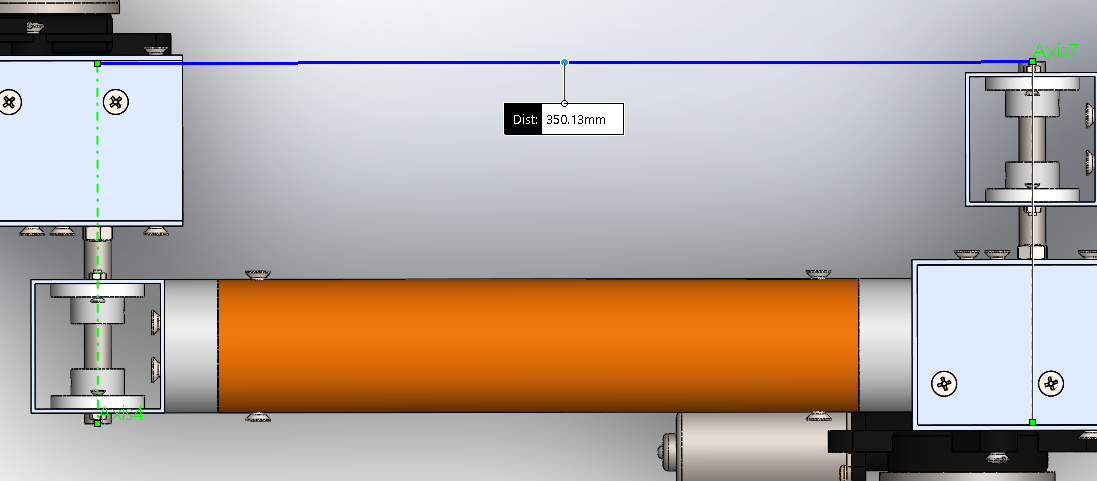
\includegraphics[width=0.9\columnwidth]{adendo/images/a3.png}
    
    \par\end{centering}

    \label{fig:a3}
\end{figure}

\begin{figure}[ht]
    \caption{Distância entre os eixos das juntas 4 e 5.}    
    \begin{centering}

        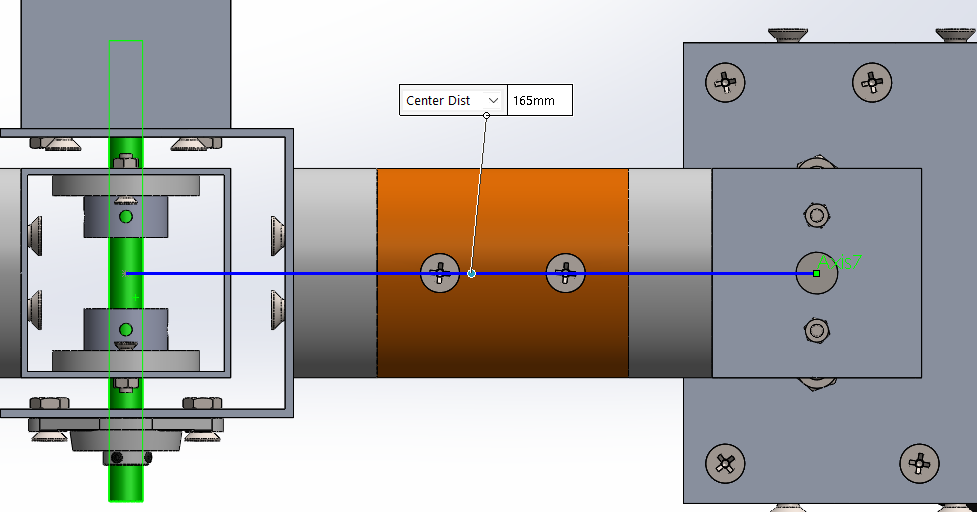
\includegraphics[width=0.9\columnwidth]{adendo/images/a4.png}
    
    \par\end{centering}

    \label{fig:a4}
\end{figure}

Para o sistema de coornadas da base, $\{0\}$, este foi posicionado a uma distância $d_1$ do sistema ${1}$, 
visando facilitar uma transformação entre a base do sistema e um sistema de referência global
da estação de uso real do manipulador. 
Como é definido em \cite{craig2009introduction}, a posição deste sistema é arbitrário, portanto
esta decisão não fere a convenção adotada.

\newpage

Para a junta 6, a origem do sistema foi posicionada no centro do eixo de saída do manipulador empregado nesta 
junta, assumindo que esta decisão tornaria mais simples uma definição da transformação entre a ferramenta a 
ser utilizada no manipulador e a última junta do sistema. Esta decisão resultou em um parâmetro $d_6$, que 
indica a distância entre $\hat{X}_5$ e $\hat{X}_6$ ao longo de $\hat{Z}_6$, respeitando a convenção adotada.
O valor deste parâmetro pode ser visto na figura \ref{fig:d6}.

\begin{figure}[ht]
    \caption{Distância entre o eixo da junta 5 e a origem do sistema da junta 6.}    
    \begin{centering}

        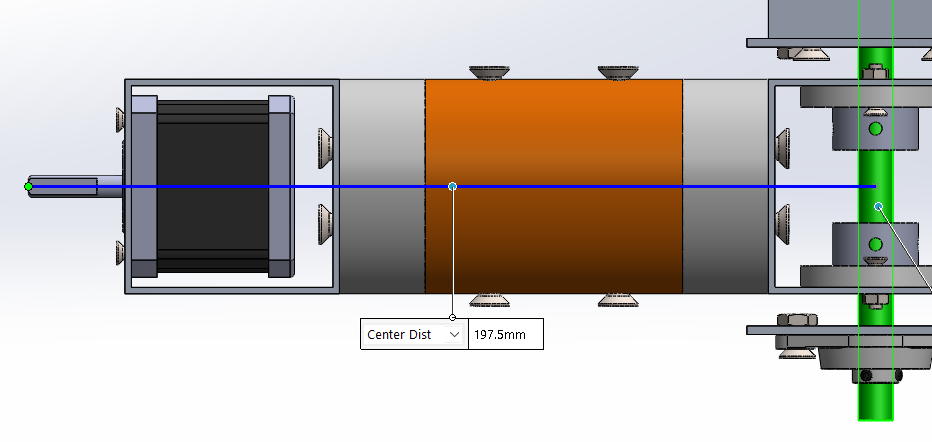
\includegraphics[width=0.9\columnwidth]{adendo/images/d6.png}
    
    \par\end{centering}

    \label{fig:d6}
\end{figure}

O modelo lógico com todos os parâmetros resultante de análise do modelo no ambiente 3D
pode ser visto na figura \ref{fig:DH-Apendice}.

\begin{figure}[ht]
    \caption{Novo modelo Denavit-Hartenberg.}    
    \begin{centering}

        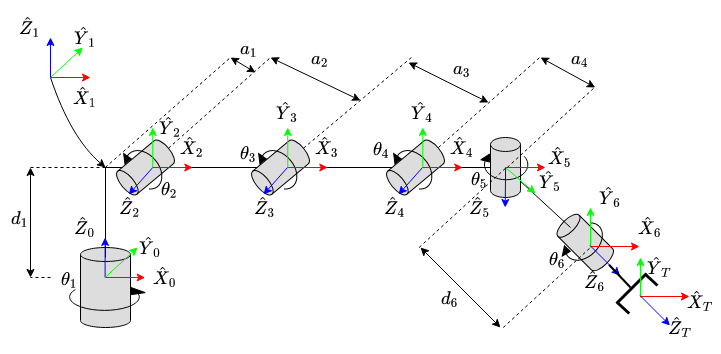
\includegraphics[width=0.9\columnwidth]{images/arm/Refframes2.png}
    
    \par\end{centering}

    \label{fig:DH-Apendice}
\end{figure}